%%%%%%%%%%%%%%%%%%%%%%%%%%%%%%%%%%%%%%%%%%%%%%%%%%%%%%%%%%%%%%%%%%%%%%%%%%%%%%%%%
\chapter{解集合プログラミング}\label{chap:asp}
%%%%%%%%%%%%%%%%%%%%%%%%%%%%%%%%%%%%%%%%%%%%%%%%%%%%%%%%%%%%%%%%%%%%%%%%%%%%%%%%%
この章では,前章で挙げた諸問題を解くために利用した
解集合プログラミング(Answer Ser Programming; ASP
\cite{%
  Hayama17,%
  Inoue08}
)
について,主にその言語とASPシステムについて解説する.
解集合プログラミングは,
非単調論理プログラミングが制約プログラミング(Constraint Programming; CP)の概念と融合した
論理プログラミングの枠組みである.\cite{Inoue08}
そして,その記述言語は,一階論理に基づく知識表現言語の一種であり,一般拡張選言プログラム(GEDP)かそのサブクラスをベースとしているが,
本論文では簡単のため,GEDPのサブクラスである\textbf{標準論理プログラム}(Normal Logic Program; NLP)を説明する.

NLPは次の形式のルールの集合である.\\
\begin{equation}
  \label{nlp:rule}
l_1 ~\mcode{:-} ~l_2, ~..., ~l_m, ~not ~l_{m+1}, ~..., ~not ~l_{n}.
\end{equation}
上記(\ref{nlp:rule})において,$0 \leq m \leq n$であり,
$l_i$は正リテラル(アトム),$not$は\textbf{デフォルトの否定}\cite{Sakama10},”$,$”は連言である.
”$\mcode{:-}$”について,左辺が\textbf{ヘッド},右辺が\textbf{ボディ}と呼ばれ,
ルール(\ref{nlp:rule})の直感的な意味は,
『$l_2, ~..., ~l_m$が全て成り立ち,$l_{m+1}, ~..., ~l_{n}$が全て成り立たないならば,$l_1$が成り立つ』
である.

(\ref{nlp:rule})で表されるルールの内,以下のようにボディが空のものは\textbf{ファクト}と呼ばれ,
”$\mcode{:-}$”を省略することができる.
ファクト(\ref{nlp:fact}),(\ref{nlp:fact2})はどちらも『$l_1$が成り立つ』という事実を示す.
\begin{eqnarray}
  \label{nlp:fact}
   l_1 ~&\mcode{:-}. \\
  \label{nlp:fact2}
   l_1.&
\end{eqnarray}

一方で,以下のようにヘッドが空であるルールは\textbf{一貫性制約}と呼ばれる.
\begin{equation}
  \mcode{:-} ~l_2, ~..., ~l_m, ~not ~l_{m+1}, ~..., ~not ~l_{n}.
\end{equation}
例えば,一貫性制約(\ref{nlp:cons})は『$b$が成り立ってはならない』という制約を,
(\ref{nlp:cons2})は『$b$が成り立たなければならない』という制約をそれぞれ示す.
\begin{eqnarray}
  \label{nlp:cons}
   \mcode{:-}& ~b.\\
  \label{nlp:cons2}
   \mcode{:-}& ~not ~b.
\end{eqnarray}

さらに,本研究にて用いたものを含む最新のASP言語には,
\textbf{アグリゲート}という表記法が実装されており,組み合わせ問題を簡潔に記述することができる.
例えば,\textbf{選択子}(\ref{choice})を使うことで,集合$\{l_1, ~..., ~l_k\}$の任意の部分集合を
後述の\textbf{解集合}に含むことを指定できる.さらに,以下(\ref{numcon})のようにこの選択子の左右に数字を指定することで,
選択子が選択可能なリテラル個数の上下限を指定することができる.$ln$が下限で,$mn$が上限である.
\begin{eqnarray}
  \label{choice}
  \{l_1, ~.&.&., ~l_k\} \\
  \label{numcon}
  ln ~\{l_1, ~.&.&., ~l_k\} ~mn
\end{eqnarray}

また,先述の最短ハミルトン路・閉路問題のような組合せ最適化問題の実装時には,
最小化関数$\#minimize$や最大化関数$\#maximize$を用いることができる.
さらに,先述の制約付きハミルトン路問題を解くにあたり必要であった目的関数値の制約は,
\textbf{重み付き個数制約}”$\#sum\{w_1:l_1; ~...;~w_k:l_k\} < c$”を用いて実装した.
これは,$l_i$に対応する重み$w_i$について,値が真となるリテラル$l_i$の重みの総和がcより小さいという制約である.

ASPシステムは,与えられたGEDPやNLPから,そこに書かれた全てのルールを満たすように,安定モデル意味論
\cite{%
  Inoue08,%
  Gelfond88%
}
に基づく解集合を計算するシステムである.本研究では,ASPシステム \clingo を使用した.
 \clingo は グラウンダー \gringo とASPソルバー \clasp から構成され,
 \gringo は \clingo に与えられた一階ASPプログラムを命題ASPプログラムに変換する\textbf{基礎化}
を行った後に基礎化後のプログラムを \clasp に渡し,その後, \clasp が解集合を算出する.
\newpage
%% \[
%% %\tabcolsep = 2mm
%% \begin{array}{c|c|c|c}
%%        X                   & \reduct{P}{X}  & 
%% \reduct{P}{X}\textrm{の最小モデル}  & X\textrm{は}P\textrm{の解集合?}\\\hline
%% \{\phantom{p         ,q}\} & \{p\leftarrow,\quad q\leftarrow\}             & \{p,q\}    
%% &  \times \\\hline
%% \{         p\phantom{,q}\} & \{p\leftarrow\phantom{\quad q\leftarrow}\}    & \{p\}      
%% & \circ \\\hline
%% \{\phantom{p,}        q \} & \{\phantom{p\leftarrow,\quad} q \leftarrow\}  & \{q\}      
%% & \circ \\\hline
%% \{         p         ,q \} & \{\phantom{p\leftarrow,\quad q\leftarrow}\}   & \emptyset  
%% & \times \\\hline
%% \end{array}
%% \]

%% %%%%%%%%%%%%%%%%%%%%%%%%%%%%%%%%%
%% \begin{table}[tb]
%%   \centering
%%   \begin{tabular}{l|*{4}{p{1cm}}}
%%     論理プログラム &   $\leftarrow$ & $,$        & $;$        & $\sim$       \\\hline
%%     ソースコード   &   \texttt{:-}  & \texttt{,} & \texttt{;} & \texttt{not}
%%   \end{tabular}
%%   \caption{論理プログラムとソースコードの対応}
%%   \label{tbl:map}
%% \end{table}
%% %%%%%%%%%%%%%%%%%%%%%%%%%%%%%%%%%
%% \begin{figure}[tb]
%%   \centering
%%   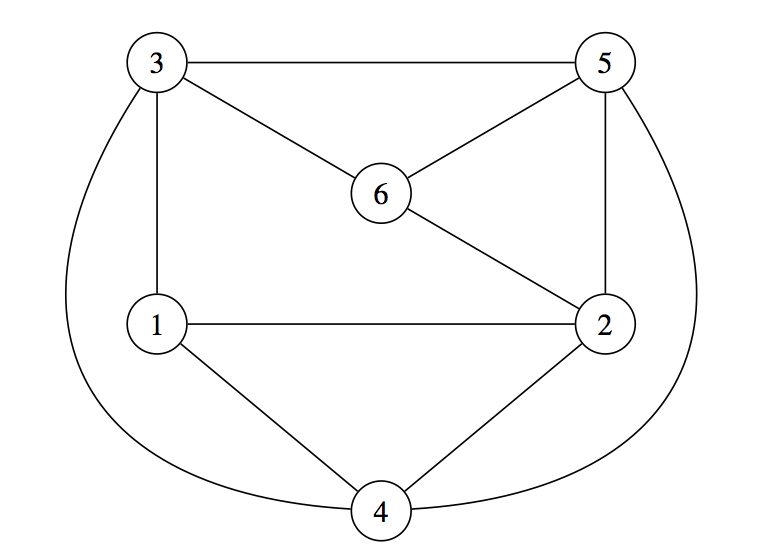
\includegraphics[width=0.6\linewidth]{fig/graph.png}
%%   \caption{グラフ}
%%   \label{fig:graph}
%% \end{figure}
%% %%%%%%%%%%%%%%%%%%%%%%%%%%%%%%%%%
%% \lstinputlisting[float=t,caption={%
%% グラフ彩色問題の論理プログラム (\code{color.lp})},%
%% captionpos=b,frame=single,label=code:color.lp,%
%% numbers=left,%
%% breaklines=true,%
%% columns=fullflexible,keepspaces=true,%
%% basicstyle=\ttfamily\scriptsize]{code/color.lp}
%% %%%%%%%%%%%%%%%%%%%%%%%%%%%%%%%%%
%% \lstinputlisting[float=t,caption={%
%% \code{color.lp}に対する{\clingo}の実行例},%
%% captionpos=b,frame=single,label=code:color.log,%
%% numbers=none,%
%% breaklines=true,%
%% columns=fullflexible,keepspaces=true,%
%% basicstyle=\ttfamily\scriptsize]{code/color.log}
%% %%%%%%%%%%%%%%%%%%%%%%%%%%%%%%%%%

%%% Local Variables:
%%% mode: japanese-latex
%%% TeX-master: "paper"
%%% End:
